\subsection{Quản lý công tác}
\label{subsec:req_business_trip}
\label{subsec:module_business_trip}

\subsubsection{Mục tiêu và yêu cầu chức năng}

Chức năng quản lý công tác hỗ trợ cán bộ, giảng viên thực hiện các nghiệp vụ liên quan đến kế hoạch đi công tác (trong nước hoặc nước ngoài, cá nhân hoặc theo đoàn) trên MyHCMUT Mobile: khởi tạo hồ sơ, khai báo kế hoạch và dự toán kinh phí, đính kèm giấy mời, theo dõi tiến trình phê duyệt, thu hồi hoặc điều chỉnh hồ sơ khi có yêu cầu.

Tương tự nghiệp vụ nghỉ phép, việc phê duyệt hồ sơ công tác được tổ chức theo quy trình nhiều cấp tùy thuộc vào tính chất chuyến đi (công tác trong nước do lãnh đạo đơn vị và Phòng TCCB phê duyệt; công tác nước ngoài hoặc chuyến đi của lãnh đạo yêu cầu thẩm quyền phê duyệt của Ban Giám hiệu). Hệ thống máy chủ HRM là nơi kiểm soát độc lập tính hợp lệ của thời gian biểu (kiểm tra xung đột với lịch nghỉ phép hoặc các chuyến công tác khác), xác thực thẩm quyền của từng cấp xử lý và quản lý chuyển đổi trạng thái hồ sơ.

Bảng~\ref{tab:fr_business_trip} tổng hợp các yêu cầu chức năng của nhóm quản lý công tác.

\begin{table}[H]
\centering
\small
\caption{Yêu cầu chức năng nhóm quản lý công tác}
\label{tab:fr_business_trip}
\begin{tabularx}{\textwidth}{|L{1.8cm}|L{3.5cm}|L{2.5cm}|Y|}
\hline
\textbf{Mã FR} & \textbf{Chức năng} & \textbf{Tác nhân} & \textbf{Mô tả và ràng buộc nghiệp vụ} \\
\hline
FR-BTR-01 & Tra cứu hồ sơ & Cán bộ, Giảng viên & Xem danh sách hồ sơ công tác cá nhân, lọc theo trạng thái và xem chi tiết tiến trình duyệt. \\
\hline
FR-BTR-02 & Lập và nộp hồ sơ & Cán bộ, Giảng viên & Nhập liệu qua wizard 5 bước: thông tin chung, kế hoạch, thành phần, kinh phí, minh chứng; lưu nháp hoặc gửi duyệt. \\
\hline
FR-BTR-03 & Điều chỉnh và thu hồi & Cán bộ, Giảng viên & Thu hồi hồ sơ khi chưa được tiếp nhận xử lý; chỉnh sửa và nộp lại hồ sơ bị trả lại. \\
\hline
FR-BTR-04 & Phê duyệt theo thẩm quyền & Cấp phê duyệt & Xem xét tờ trình, minh chứng và phê duyệt, từ chối hoặc trả lại hồ sơ theo thẩm quyền phân công. \\
\hline
\end{tabularx}
\end{table}

\subsubsection{Đặc tả Use Case}

Các use case của nhóm quản lý công tác mô tả quá trình từ khi cán bộ khởi tạo hồ sơ, hoàn thiện các bước nội dung, gửi xử lý, theo dõi cho đến khi được cấp có thẩm quyền ra quyết định phê duyệt. Hình~\ref{fig:uc_business_trip} thể hiện sơ đồ use case của nhóm quản lý công tác.

\begin{figure}[H]
\centering
\fbox{\parbox[c][5.5cm][c]{0.85\linewidth}{\centering \textbf{Sơ đồ Đặc tả Use case Quản lý công tác} \newline \textit{(Gồm tác nhân Cán bộ/Giảng viên, Lãnh đạo Đơn vị, Lãnh đạo Phòng TCCB, Ban Giám hiệu và các use case UC-BTR-01 đến UC-BTR-03)}}}
\caption{Sơ đồ Đặc tả Use case nhóm Quản lý công tác}
\label{fig:uc_business_trip}
\end{figure}

Bảng~\ref{tab:mapping_uc_btr} tổng hợp danh mục các use case thuộc nhóm quản lý công tác.

\begin{table}[H]
\centering
\small
\caption{Danh mục Đặc tả Use casenhóm Quản lý công tác}
\label{tab:mapping_uc_btr}
\vspace{0.15cm}
\begin{tabularx}{\textwidth}{|L{2.6cm}|L{4.5cm}|Y|}
\hline
\textbf{Mã Use Case} & \textbf{Tên Use Case} & \textbf{Mục tiêu Nghiệp vụ} \\
\hline
\textbf{UC-BTR-01} & Quản lý hồ sơ công tác cá nhân & Tra cứu danh sách, xem chi tiết tiến trình phê duyệt, thu hồi hoặc chỉnh sửa hồ sơ. \\
\hline
\textbf{UC-BTR-02} & Lập và gửi hồ sơ công tác & Khởi tạo hồ sơ qua wizard 5 bước, kiểm tra trùng lịch và gửi phê duyệt. \\
\hline
\textbf{UC-BTR-03} & Xử lý hồ sơ công tác & Xem xét tờ trình, thẩm định kinh phí/minh chứng và phê duyệt, từ chối hoặc trả lại hồ sơ. \\
\hline
\end{tabularx}
\end{table}

Hai use case cốt lõi làm thay đổi trạng thái hồ sơ là \textbf{UC-BTR-02} và \textbf{UC-BTR-03} được đặc tả chi tiết tại Bảng~\ref{tab:uc_btr_02} và Bảng~\ref{tab:uc_btr_03}. Đặc tả Use Case \textbf{UC-BTR-01} được đặc tả tại Bảng~\ref{tab:uc_btr_01}.

\usecasespec{
  id={UC-BTR-01},
  name={Quản lý hồ sơ công tác cá nhân},
  shortname={Quản lý hồ sơ cá nhân},
  actor={Cán bộ / Giảng viên},
  desc={Cho phép cán bộ tra cứu danh sách hồ sơ công tác theo trạng thái, xem tiến trình luân chuyển, thu hồi hồ sơ đang chờ duyệt hoặc chỉnh sửa hồ sơ bị trả lại.},
  pre={Cán bộ đã đăng nhập thành công vào ứng dụng MyHCMUT Mobile.},
  trigger={Người dùng chọn mục ``Đi công tác'' trên giao diện ứng dụng.},
  mainflow={
    1. Người dùng mở mục ``Đi công tác'' để xem danh sách hồ sơ đã tạo. \newline
    2. Người dùng lọc danh sách hoặc chọn một hồ sơ để xem nội dung và trạng thái xử lý. \newline
    3. Với hồ sơ đang chờ xử lý, người dùng có thể yêu cầu thu hồi. \newline
    4. HRM kiểm tra trạng thái hiện tại và ghi nhận kết quả thu hồi khi hợp lệ.
  },
  altflow={
    - \textit{Luồng 3a (Sửa hồ sơ bị trả lại):} Với hồ sơ ở trạng thái Bị trả lại, người dùng chọn chỉnh sửa theo ý kiến cấp duyệt và nộp lại.
  },
  exflow={
    - \textit{Ngoại lệ 4a (Hồ sơ đã tiếp nhận xử lý):} Cấp duyệt đã tiếp nhận hoặc phê duyệt hồ sơ $\rightarrow$ hệ thống từ chối thu hồi và làm mới danh sách.
  },
  post={Cán bộ nắm bắt chính xác tiến trình xử lý hồ sơ; trạng thái thu hồi hoặc điều chỉnh được cập nhật đồng bộ.},
  label={tab:uc_btr_01}
}

\usecasespec{
  id={UC-BTR-02},
  name={Lập và gửi hồ sơ công tác},
  shortname={Lập và gửi hồ sơ công tác},
  actor={Cán bộ / Giảng viên},
  desc={Cho phép cán bộ lập mới hồ sơ công tác qua biểu mẫu hướng dẫn 5 bước, kiểm tra xung đột thời gian biểu, khai báo nhân sự, kinh phí, đính kèm minh chứng và nộp duyệt.},
  pre={Cán bộ đã đăng nhập vào hệ thống và có quyền lập hồ sơ công tác.},
  trigger={Người dùng nhấn nút tạo mới hồ sơ công tác trên giao diện ứng dụng.},
  mainflow={
    1. Người dùng chọn tạo mới hồ sơ công tác; ứng dụng kiểm tra ngày đăng ký có hợp lệ trước khi yêu cầu tạo nháp. \newline
    2. Khi ngày đăng ký hợp lệ, hệ thống khởi tạo bản ghi nháp. \newline
    3. Người dùng nhập thông tin chuyến đi, kế hoạch, thành phần, kinh phí và minh chứng theo loại hồ sơ. \newline
    4. Người dùng rà soát thông tin và gửi hồ sơ. \newline
    5. HRM kiểm tra các điều kiện nghiệp vụ, bao gồm xung đột lịch, và tiếp nhận hồ sơ hợp lệ vào quy trình luân chuyển.
  },
  altflow={
    - \textit{Luồng 3a (Lưu nháp):} Người dùng chọn lưu hồ sơ ở trạng thái nháp tại bất kỳ bước nào để tiếp tục hoàn thiện sau.
  },
  exflow={
    - \textit{Ngoại lệ 1a (Ngày đăng ký không hợp lệ):} Ứng dụng thông báo nguyên nhân và không tạo bản ghi nháp. \newline
    - \textit{Ngoại lệ 3a (Xung đột thời gian biểu):} Thời gian công tác trùng lặp với lịch nghỉ phép hoặc lịch công tác khác $\rightarrow$ hệ thống cảnh báo và yêu cầu điều chỉnh. \newline
    - \textit{Ngoại lệ 3b (Thiếu minh chứng bắt buộc):} Chuyến đi yêu cầu giấy mời bắt buộc chưa được đính kèm $\rightarrow$ hệ thống từ chối nộp duyệt.
  },
  post={Hồ sơ hợp lệ được chuyển sang bước xử lý tương ứng; nháp có thể tiếp tục hoàn thiện theo quyền.},
  label={tab:uc_btr_02}
}

\usecasespec{
  id={UC-BTR-03},
  name={Xử lý hồ sơ công tác},
  shortname={Xử lý hồ sơ công tác},
  actor={Lãnh đạo Đơn vị, Lãnh đạo Phòng TCCB, Ban Giám hiệu},
  desc={Cho phép cấp có thẩm quyền xem xét tờ trình, thẩm định kinh phí, minh chứng và phê duyệt, từ chối hoặc trả lại hồ sơ công tác ở bước được phân công.},
  pre={Tài khoản có quyền xử lý và hồ sơ đang chờ tại bước tương ứng trong quy trình luân chuyển.},
  trigger={Người xử lý mở danh sách hồ sơ chờ xử lý trên ứng dụng hoặc từ thông báo nhắc việc.},
  mainflow={
    1. Người xử lý mở danh sách hồ sơ công tác chờ xử lý thuộc thẩm quyền phân công. \newline
    2. Chọn xem chi tiết một hồ sơ để kiểm tra nội dung và minh chứng liên quan. \newline
    3. Người xử lý lựa chọn hành động: \textit{Phê duyệt}, \textit{Từ chối} hoặc \textit{Trả lại}. \newline
    4. HRM kiểm tra quyền và trạng thái hồ sơ hiện tại, rồi ghi nhận kết quả xử lý hoặc chuyển hồ sơ sang bước tiếp theo. \newline
    5. Hệ thống thông báo kết quả xử lý cho các bên liên quan.
  },
  altflow={
    - \textit{Luồng 3a (Trả lại yêu cầu hoàn thiện):} Người duyệt chọn ``Trả lại'' kèm ý kiến chỉ đạo $\rightarrow$ hồ sơ chuyển về trạng thái Bị trả lại.
  },
  exflow={
    - \textit{Ngoại lệ 3a (Từ chối hồ sơ):} Người duyệt bắt buộc nhập lý do từ chối trước khi hệ thống ghi nhận kết quả. \newline
    - \textit{Ngoại lệ 4a (Hồ sơ đã thay đổi trạng thái):} Hồ sơ đã bị thu hồi hoặc xử lý bởi cấp khác $\rightarrow$ hệ thống không ghi nhận thao tác và làm mới danh sách.
  },
  post={Hồ sơ chuyển sang trạng thái phản ánh kết quả xử lý hợp lệ tại thời điểm thao tác.},
  label={tab:uc_btr_03}
}

\subsubsection{Biểu đồ hoạt động}

Quy trình quản lý công tác bao gồm hai luồng xử lý chính: luồng lập và nộp hồ sơ của cán bộ và luồng luân chuyển phê duyệt đa cấp theo thẩm quyền.

Hình~\ref{fig:act_trip_submit} mô tả quy trình lập và gửi hồ sơ công tác (UC-BTR-02). Quy trình thể hiện rõ các bước tuần tự qua wizard 5 bước: khai báo thông tin $\rightarrow$ kế hoạch $\rightarrow$ thành phần $\rightarrow$ tài chính/minh chứng $\rightarrow$ rà soát nộp.

\begin{figure}[H]
\centering
\fbox{\parbox[c][7cm][c]{0.85\linewidth}{\centering \textbf{Biểu đồ hoạt động: Quy trình lập và gửi hồ sơ công tác} \newline \textit{(Chi tiết quy trình wizard 5 bước: Thông tin chung $\rightarrow$ Kế hoạch $\rightarrow$ Thành phần đoàn $\rightarrow$ Kinh phí \& Minh chứng $\rightarrow$ Nộp duyệt)}}}
\caption{Biểu đồ hoạt động Quy trình lập và gửi hồ sơ công tác}
\label{fig:act_trip_submit}
\end{figure}

Hình~\ref{fig:act_trip_approve} mô tả quy trình luân chuyển phê duyệt hồ sơ công tác đa cấp (UC-BTR-03). Quy trình thể hiện các cấp thẩm quyền (Lãnh đạo đơn vị $\rightarrow$ Phòng TCCB $\rightarrow$ Ban Giám hiệu) và các nhánh xử lý (Phê duyệt, Trả lại bổ sung, Từ chối kèm lý do).

\begin{figure}[H]
\centering
\fbox{\parbox[c][7cm][c]{0.85\linewidth}{\centering \textbf{Biểu đồ hoạt động: Quy trình phê duyệt hồ sơ công tác đa cấp} \newline \textit{(Thể hiện các làn bơi thẩm quyền: Lãnh đạo Đơn vị $\leftrightarrow$ Phòng TCCB $\leftrightarrow$ Ban Giám hiệu; luân chuyển theo loại chuyến đi)}}}
\caption{Biểu đồ hoạt động Quy trình phê duyệt hồ sơ công tác đa cấp}
\label{fig:act_trip_approve}
\end{figure}

\subsubsection{Biểu đồ tuần tự}

Biểu đồ tuần tự mô tả sự phối hợp ở mức logic giữa Người dùng, MyHCMUT Mobile và Hệ thống HRM trong kịch bản Lập và gửi hồ sơ công tác (UC-BTR-02). Biểu đồ thể hiện trình tự khởi tạo nháp, kiểm tra xung đột lịch trình và tiếp nhận hồ sơ vào quy trình luân chuyển.

Hình~\ref{fig:seq_trip_submit} thể hiện biểu đồ tuần tự của use case Gửi hồ sơ công tác.

\begin{figure}[H]
\centering
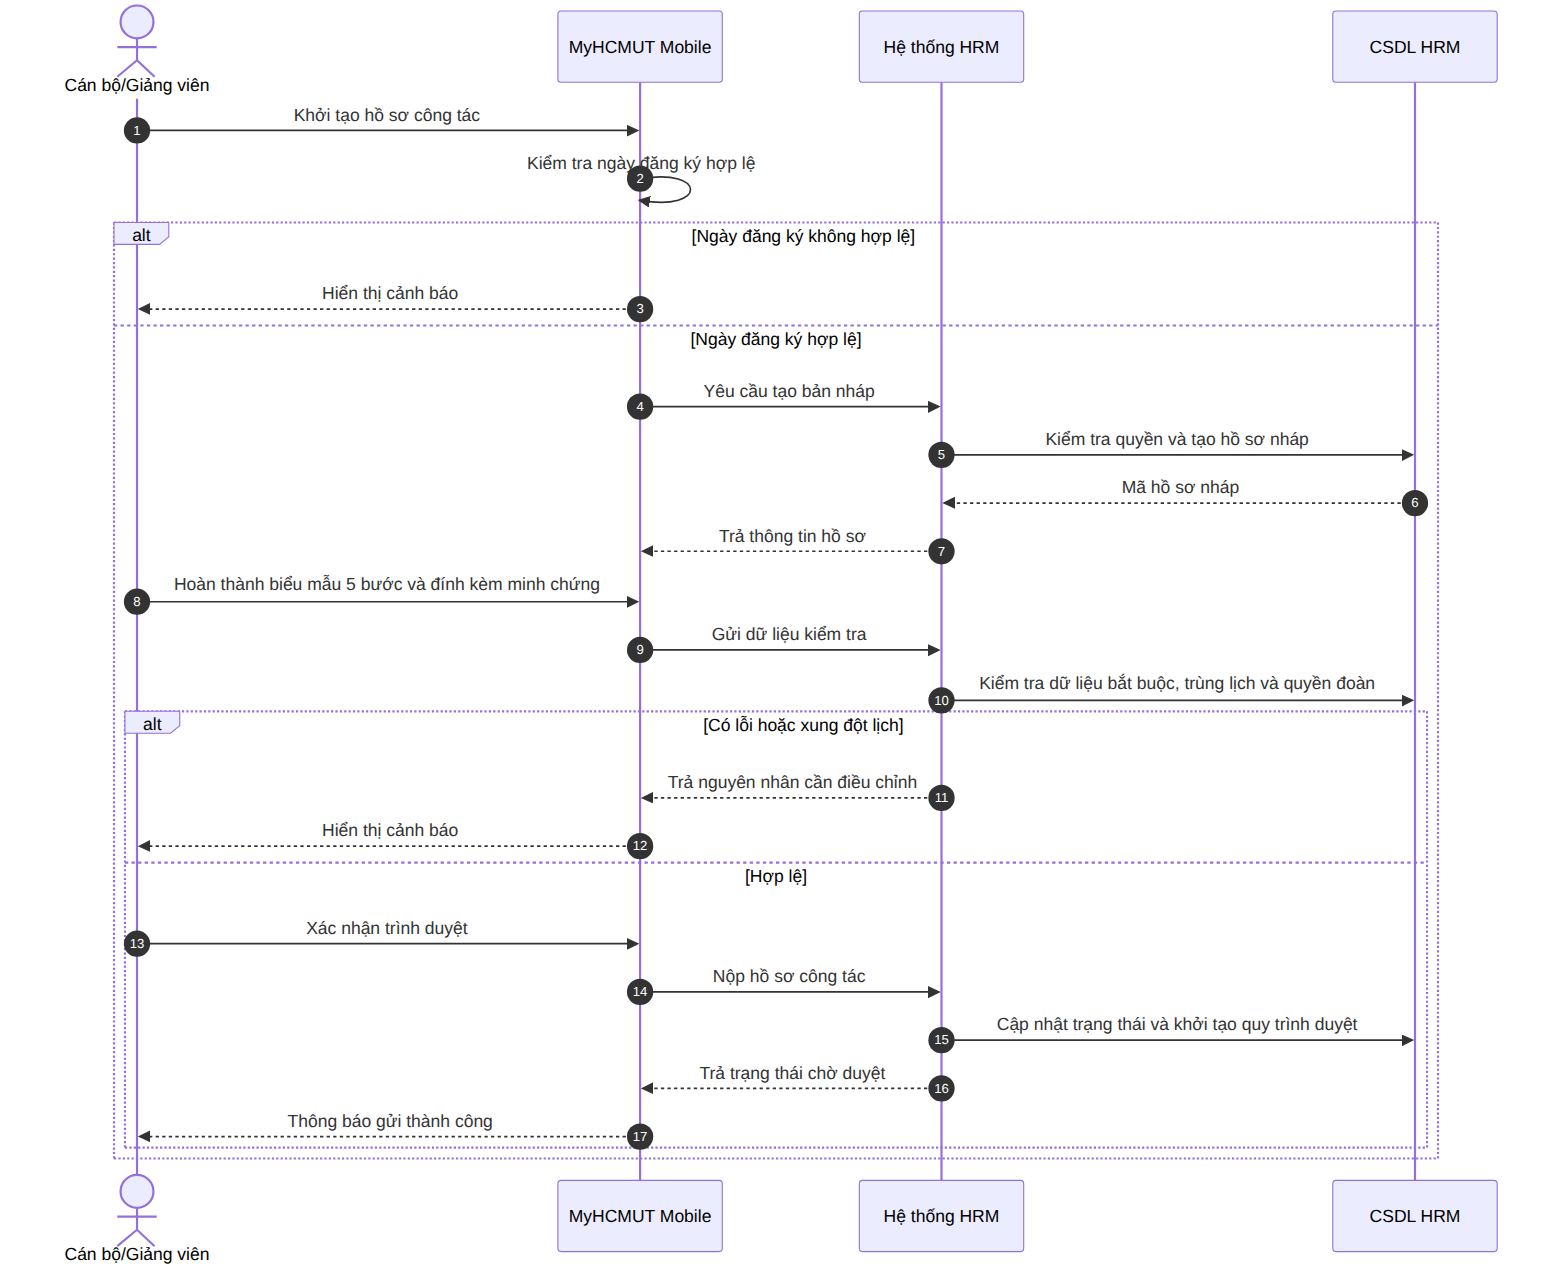
\includegraphics[width=\linewidth]{image/uml/seq_trip_submit.png}
\caption{Biểu đồ tuần tự Gửi hồ sơ công tác}
\label{fig:seq_trip_submit}
\end{figure}
